% Unit 062 English translation of chapter4.tex lines 2268--2499.
% Source: Methods of Algebra, Volume 2, commit
% 9a5803ff77dd3257484cb177f851a73770a59dd3 (CC BY 4.0).
% stable-unit-id: o014.aljabr2.chapter4.k-flat-derived-tensor-a
% Coverage: first half of Section 4.12, on K-flat complexes, K-flat
% resolutions, and the construction of the derived tensor product; stops
% after the paragraph at line 2499, just before the corollary at line 2500.

% segment-id: o014.li2.chapter4.k-flat-derived-tensor-a.h001
\section{Example: K-Flat Complexes and \texorpdfstring{$\otimesL$}{otimesL}}\label{sec:otimesL}
\hypertarget{o014.aljabr2.chapter4.k-flat-derived-tensor-a}{ }

% segment-id: o014.li2.chapter4.k-flat-derived-tensor-a.p001
Throughout this section, $\Bbbk$ is a commutative ring.

% segment-id: o014.li2.chapter4.k-flat-derived-tensor-a.cv001
\begin{convention}\label{con:bimodule-algebra}
	Let $R$ and $S$ be $\Bbbk$-algebras. By the convention of this book, every
	$(R,S)$-bimodule $M$ is tacitly assumed to satisfy $tm=mt$ for
	$t\in\Bbbk$ and $m\in M$. In other words,
	$(R,S)\dcate{Mod}\simeq(R\dotimes{\Bbbk}S^{\opp})\dcate{Mod}$. When
	$\Bbbk=\Z$, this condition is redundant.

	From now on, the forgetful functor
	$(R,S)\dcate{Mod}\to R\dcate{Mod}$ (respectively,
	$(R,S)\dcate{Mod}\to\cated{Mod}S$) is written
	$M\mapsto{}_RM$ (respectively, $M\mapsto M_S$); the same notation applies
	to complexes. These forgetful functors are exact, and the triangulated
	functors they induce between derived categories are denoted in the same way.
\end{convention}

% segment-id: o014.li2.chapter4.k-flat-derived-tensor-a.p002
Notice that, for every complex $M$ of $(R,S)$-bimodules, one has
% segment-id: o014.li2.chapter4.k-flat-derived-tensor-a.q001
\[ M_S \;\text{acyclic} \iff M \;\text{acyclic} \iff {}_R M \;\text{acyclic}. \]

% segment-id: o014.li2.chapter4.k-flat-derived-tensor-a.p003
From now on, let $R$, $A$, and $B$ be $\Bbbk$-algebras. Our starting point is
the bifunctor given by the tensor product,
% segment-id: o014.li2.chapter4.k-flat-derived-tensor-a.q002
\[ \otimes_R: (A, R)\dcate{Mod} \times (R, B)\dcate{Mod} \to (A, B)\dcate{Mod}, \]
which is right exact in each variable. The simplest case is $A=\Bbbk=B$; the
corresponding bifunctor becomes
$\otimes_R:\cated{Mod}R\times R\dcate{Mod}\to\cate{\Bbbk}$.

% segment-id: o014.li2.chapter4.k-flat-derived-tensor-a.p004
For convenience, if $X$ is a complex of $(A,R)$-bimodules and $Y$ is a
complex of $(R,B)$-bimodules, we henceforth write the bicomplex obtained by
taking tensor products term by term as
$X^\bullet\dotimes{R}Y^\bullet$, and write its total complex as
% segment-id: o014.li2.chapter4.k-flat-derived-tensor-a.q003
\[ X \dotimes{R} Y := \tot_{\oplus} \left( X^\bullet \dotimes{R} Y^\bullet \right). \]

% segment-id: o014.li2.chapter4.k-flat-derived-tensor-a.p005
Categories of bimodules have enough K-projective complexes (apply
Example~\ref{eg:Mod-K-injectives}); hence
Proposition~\ref{prop:bifunctor-via-K-injective} ensures the existence of the
unbounded left derived bifunctor.

% segment-id: o014.li2.chapter4.k-flat-derived-tensor-a.d001
\begin{definition}\label{def:otimesL}
	\index{derived tensor product}
	\index[sym1]{XotimesLY@$X \otimesL[R] Y$}
	Denote the left derived bifunctor
	$\mathrm{L}\left(\cdot\dotimes{R}\cdot\right)$ of $\otimes_R$ by
% segment-id: o014.li2.chapter4.k-flat-derived-tensor-a.q004
	\[ \otimesL[R] : \cate{D}((A, R)\dcate{Mod}) \times \cate{D}((R, B)\dcate{Mod}) \to \cate{D}((A, B)\dcate{Mod}). \]
	When no confusion can arise, $X\otimesL[R]Y$ is also abbreviated to
	$X\otimesL Y$.
\end{definition}

% segment-id: o014.li2.chapter4.k-flat-derived-tensor-a.p006
The abstract definition above is straightforward, but to study $\otimes_R$
further we still need to introduce a class of quasi-isomorphisms called K-flat
resolutions. The reasons include the following:
% segment-id: o014.li2.chapter4.k-flat-derived-tensor-a.l001
\begin{itemize}
% segment-id: o014.li2.chapter4.k-flat-derived-tensor-a.i001
	\item the definition of a K-flat resolution is directly related to the tensor
	product and is more useful for establishing important properties and making
	concrete computations, as already seen in \S\ref{sec:Ext-Tor};
% segment-id: o014.li2.chapter4.k-flat-derived-tensor-a.i002
	\item in geometric settings such as sheaf theory, K-injective resolutions
	may be available while K-projective resolutions are not; in that situation,
	K-flat resolutions are the only means of studying the derived tensor product.
\end{itemize}

% segment-id: o014.li2.chapter4.k-flat-derived-tensor-a.d002
\begin{definition}[N.\ Spaltenstein {\cite[Definition 5.1]{Spa88}}]
	\index{complex!K-flat}
	Let $X$ be a complex of right $R$-modules. If, for every complex $Y$ of
	left $R$-modules,
% segment-id: o014.li2.chapter4.k-flat-derived-tensor-a.q005
	\[ Y \;\text{acyclic} \implies X \dotimes{R} Y\;\text{acyclic}, \]
	then $X$ is called \emph{K-flat}\footnote{A more reasonable name might be a
	homotopy-flat complex.}; this property depends only on the isomorphism class
	of $X$ in $\cate{K}(\cated{Mod}R)$. K-flatness is defined similarly for
	complexes of left $R$-modules.
\end{definition}

% segment-id: o014.li2.chapter4.k-flat-derived-tensor-a.p007
For bounded-above complexes, K-flatness follows from the familiar notion of
flatness in module theory.

% segment-id: o014.li2.chapter4.k-flat-derived-tensor-a.pr001
\begin{proposition}\label{prop:flat-K-flat}
	Let $X$ be an object of $\cate{C}^-(\cated{Mod}R)$, and suppose that every
	$X^n$ is flat. Then $X$ is K-flat. The same statement holds for objects of
	$\cate{C}^-(R\dcate{Mod})$.
\end{proposition}

% segment-id: o014.li2.chapter4.k-flat-derived-tensor-a.pf001
\begin{proof}
	Let $Y$ be an acyclic complex of left $R$-modules; we shall prove that
	$X\dotimes{R}Y$ is acyclic. Using truncation functors, write $Y$ as
	$\varinjlim_m\tau^{\leq m}Y$. Degree by degree, $\varinjlim_m$ commutes
	both with tensor products \cite[Proposition 6.9.2]{Li1} and with
	$\bigoplus$; it therefore suffices to consider the case in which $Y$ is
	bounded above. Then $X^\bullet\dotimes{R}Y^\bullet$ belongs to the category
	$\cate{C}^2_f(\Bbbk\dcate{Mod})$ of Definition~\ref{def:Cf-Supp}. Since
	$X^p\dotimes{R}Y^\bullet$ is acyclic for every $p$,
	Corollary~\ref{prop:acyclic-assembly} ensures that $X\dotimes{R}Y$ is
	acyclic.
\end{proof}

% segment-id: o014.li2.chapter4.k-flat-derived-tensor-a.p008
In view of this result, if the reader is interested only in bounded-above
derived categories, every K-flat complex appearing in this section may be
replaced by a bounded-above complex of flat modules.

% segment-id: o014.li2.chapter4.k-flat-derived-tensor-a.d003
\begin{definition}
	\index{resolution!K-flat}
	\index{enough K-flat complexes}
	If $P\to X$ is a quasi-isomorphism in
	$\cate{C}((A,R)\dcate{Mod})$ and $P_R$ is K-flat, then this morphism is
	called a \emph{K-flat resolution} of $X$ relative to $R$. If every
	$X\in\cate{C}((A,R)\dcate{Mod})$ has a K-flat resolution relative to $R$,
	then $(A,R)\dcate{Mod}$ is said to have enough K-flat complexes relative to
	$R$.

	A K-flat resolution relative to $R$ is defined similarly for
	$X\in\Obj(\cate{C}((R,B)\dcate{Mod}))$.
\end{definition}

% segment-id: o014.li2.chapter4.k-flat-derived-tensor-a.p009
A natural question is how to guarantee that a category of bimodules has
enough K-flat complexes relative to $R$. What is the relation between K-flat
and K-projective complexes? As expected, the bridge comes from the classical
adjunction between $\otimes$ and $\Hom$ \cite[Theorem 6.6.5]{Li1}.

% segment-id: o014.li2.chapter4.k-flat-derived-tensor-a.p010
The first step is to lift that adjunction to the level of complexes. If $Y$ is
an object of $\cate{C}((R,B)\dcate{Mod})$ and $Z$ is an object of
$\cate{C}((A,B)\dcate{Mod})$, the $\Hom$ complex
$\Hom^\bullet(Y_B,Z_B)$ can be endowed degree by degree with an
$(A,R)$-bimodule structure, making it an object of
$\cate{C}((A,R)\dcate{Mod})$.

% segment-id: o014.li2.chapter4.k-flat-derived-tensor-a.pr002
\begin{proposition}[$\Hom$--$\otimes$ adjunction: complex version]\label{prop:tensor-Hom-cplx}
	Let $X$ be an object of $\cate{C}((A,R)\dcate{Mod})$, let $Y$ be an object
	of $\cate{C}((R,B)\dcate{Mod})$, and let $Z$ be an object of
	$\cate{C}((A,B)\dcate{Mod})$. There are canonical isomorphisms in
	$\cate{C}(\Bbbk\dcate{Mod})$
% segment-id: o014.li2.chapter4.k-flat-derived-tensor-a.q007
	\begin{align*}
		\Hom^\bullet\left( X \dotimes{R} Y, \; Z \right) & \simeq \Hom^\bullet\left( X, \Hom^\bullet(Y_B, Z_B) \right) \\
		& \simeq \Hom^\bullet\left( Y, \Hom^\bullet({}_A X, {}_A Z) \right).
	\end{align*}

	Consequently, taking $\Ker(d^0)$ gives isomorphisms of $\Bbbk$-modules
% segment-id: o014.li2.chapter4.k-flat-derived-tensor-a.q008
	\begin{align*}
		\Hom_{\cate{C}((A, B)\dcate{Mod})}\left( X \dotimes{R} Y, \; Z \right) & \simeq \Hom_{\cate{C}((A, R)\dcate{Mod})}\left( X, \Hom^\bullet(Y_B, Z_B) \right) \\
		& \simeq \Hom_{\cate{C}((R, B)\dcate{Mod})}\left( Y, \Hom^\bullet({}_A X, {}_A Z) \right).
	\end{align*}
\end{proposition}

% segment-id: o014.li2.chapter4.k-flat-derived-tensor-a.pf002
\begin{proof}
	It suffices to treat the first isomorphism. To simplify notation, write
	$Y$ and $Z$ for $Y_B$ and $Z_B$ below, and omit the subscript on $\Hom$.
	Fix $n\in\Z$. The degree-$n$ term on the left-hand side is
% segment-id: o014.li2.chapter4.k-flat-derived-tensor-a.e001
	\begin{multline}\label{eqn:tensor-Hom-cplx-aux}
		\prod_k \Hom\left( (X \dotimes{R} Y)^k, Z^{k+n}\right) \simeq \prod_k \prod_{p+q=k} \Hom\left(X^p \dotimes{R} Y^q, Z^{k+n}\right) \\
		= \prod_{p, q} \Hom\left( X^p \dotimes{R} Y^q, Z^{p+q+n} \right) \simeq \prod_p \prod_q \Hom\left( X^p, \Hom\left(Y^q, Z^{p+q+n}\right) \right) \\
		\simeq \prod_p \Hom\left( X^p, \Hom^{p+n}(Y, Z) \right),
	\end{multline}
	and the last term is precisely the degree-$n$ term on the right-hand side.
	Concretely, under the second isomorphism $\simeq$, the homomorphism of
	$(A,B)$-bimodules
	$\varphi^{p,q}:X^p\dotimes{R}Y^q\to Z^{p+q+n}$ corresponds to
% segment-id: o014.li2.chapter4.k-flat-derived-tensor-a.q009
	\[ \left[ x \mapsto [y \mapsto \varphi^{p,q}(x \otimes y)] \right] \; \in \Hom\left( X^p, \Hom\left(Y^q, Z^{p+q+n}\right) \right). \]
	It remains only to verify that \eqref{eqn:tensor-Hom-cplx-aux} determines an
	isomorphism of complexes.

	Take an element of the degree-$n$ term on the left and write it as
	$(\varphi^{p,q})_{p,q\in\Z}$. The $(p,q)$-component of its image under
	$d_{\Hom^\bullet(X\otimes Y,Z)}$ sends
	$x\otimes y\in X^p\dotimes{R}Y^q$ to
% segment-id: o014.li2.chapter4.k-flat-derived-tensor-a.q010
	\[ d_Z \varphi^{p,q}(x \otimes y) - (-1)^n \left( \varphi^{p+1, q}(d_X x \otimes y) + (-1)^p \varphi^{p, q+1}(x \otimes d_Y y) \right). \]

	For the corresponding element of degree $n$ on the right, the
	$p$-component of its image under
	$d_{\Hom^\bullet(X,\Hom^\bullet(Y,Z))}$ sends $x\in X^p$ to
% segment-id: o014.li2.chapter4.k-flat-derived-tensor-a.q011
	\[
		d_{\Hom^\bullet(Y, Z)}\left[ y \mapsto \varphi^{p,q}(x \otimes y) \right]_{q \in \Z} - (-1)^n \left[ y \mapsto \varphi^{p+1, q}(d_X x \otimes y) \right]_{q \in \Z};
	\]
	expanding the definition of $d^{p+n}_{\Hom^\bullet(Y,Z)}$ further, for
	the fixed pair $(p,q)$ this becomes
% segment-id: o014.li2.chapter4.k-flat-derived-tensor-a.q012
	\[ y \mapsto d_Z \varphi^{p,q}(x \otimes y) - (-1)^{p+n} \varphi^{p, q+1}(x \otimes d_Y y) - (-1)^n \varphi^{p+1, q}(d_X x \otimes y). \]
	This proves the assertion.
\end{proof}

% segment-id: o014.li2.chapter4.k-flat-derived-tensor-a.p011
We now return to the relation between K-projective and K-flat complexes.

% segment-id: o014.li2.chapter4.k-flat-derived-tensor-a.le001
\begin{lemma}\label{prop:K-projective-flat}
	Let $X$ be a K-projective complex of $(A,R)$-bimodules. If $A$ is flat as
	a $\Bbbk$-module, then $X_R$ is K-flat.

	Let $Y$ be a K-projective complex of $(R,B)$-bimodules. If $B$ is flat as
	a $\Bbbk$-module, then ${}_RY$ is K-flat.
\end{lemma}

% segment-id: o014.li2.chapter4.k-flat-derived-tensor-a.pf003
\begin{proof}
	It suffices to prove the first assertion. Take an acyclic complex $Y$ of
	left $R$-modules. Regard every left $A$-module $I$ (that is, every
	$(A,\Bbbk)$-bimodule) as a complex concentrated in degree zero.
	Proposition~\ref{prop:tensor-Hom-cplx}, with $B=\Bbbk$, gives
% segment-id: o014.li2.chapter4.k-flat-derived-tensor-a.q013
	\[ \Hom^\bullet\left(X \dotimes{R} Y, \; I\right) \simeq \Hom^\bullet\left(X, \Hom^\bullet(Y_{\Bbbk}, I_{\Bbbk}) \right). \]

	Suppose that $I$ is an injective left $A$-module. Then $I_{\Bbbk}$ is an
	injective $\Bbbk$-module, because the forgetful functor
	$A\dcate{Mod}\to\Bbbk\dcate{Mod}$ has the exact left adjoint
	$A\dotimes{\Bbbk}(\cdot)$; see
	Proposition~\ref{prop:adjoint-injective-projective} and
	\cite[Corollary 6.6.8]{Li1}. Hence the complex of $\Bbbk$-modules
	$\Hom^\bullet(Y_{\Bbbk},I_{\Bbbk})$ is acyclic. It remains acyclic as a
	complex of $(A,R)$-bimodules, so the K-projectivity of $X$ implies that
	$\Hom^\bullet(X\dotimes{R}Y,I)$ is acyclic.

	Because $I$ is injective, it is easy to see that, for every $n\in\Z$,
% segment-id: o014.li2.chapter4.k-flat-derived-tensor-a.q014
	\[ \Hom\left( \Hm^n\left( X \dotimes{R} Y \right), I\right) \simeq \Hm^{-n} \Hom^\bullet\left( X \dotimes{R} Y, \; I \right) = 0. \]

	Since every left $A$-module embeds into an injective module,
	$X\dotimes{R}Y$ must be acyclic. This proves the assertion.
\end{proof}

% segment-id: o014.li2.chapter4.k-flat-derived-tensor-a.p012
If the reader is interested only in tensor products over commutative rings,
that is, in the special case $A=R=B=\Bbbk$, or only in the case where
$\Bbbk$ is a field, all the flatness assumptions on $A$ or $B$ above are
automatically satisfied.

% segment-id: o014.li2.chapter4.k-flat-derived-tensor-a.co001
\begin{corollary}\label{prop:enough-K-flat}
	If $A$ (respectively, $B$) is flat as a $\Bbbk$-module, then
	$(A,R)\dcate{Mod}$ (respectively, $(R,B)\dcate{Mod}$) has enough K-flat
	complexes relative to $R$.
\end{corollary}

% segment-id: o014.li2.chapter4.k-flat-derived-tensor-a.p013
Taking $A=\Bbbk$ (respectively, $B=\Bbbk$) further shows that K-projective
complexes of right (respectively, left) $R$-modules are always K-flat relative
to $R$, and that $\cated{Mod}R$ (respectively, $R\dcate{Mod}$) has enough
K-flat complexes.

% segment-id: o014.li2.chapter4.k-flat-derived-tensor-a.p014
We now explain how to determine the derived functor of $\otimes_R$ by means
of K-flat resolutions. To simplify notation, all localization functors $Q$
will henceforth be suppressed.

% segment-id: o014.li2.chapter4.k-flat-derived-tensor-a.pr003
\begin{proposition}\label{prop:K-flat}
	Define the full subcategory $\mathcal{F}_{A,R}$ of
	$\cate{K}((A,R)\dcate{Mod})$ by
% segment-id: o014.li2.chapter4.k-flat-derived-tensor-a.q015
	\[ \Obj(\mathcal{F}_{A,R}) = \{ X: X_R \;\text{K-flat} \}; \]
	and define $\mathcal{F}_{R,B}$ similarly. Both are saturated triangulated
	subcategories. We now determine subcategories of
% segment-id: o014.li2.chapter4.k-flat-derived-tensor-a.q016
	\[ \cate{K}((A,R)\dcate{Mod}) \times \cate{K}((R,B)\dcate{Mod}) \quad \text{that are $\otimes_R$-projective}. \]
% segment-id: o014.li2.chapter4.k-flat-derived-tensor-a.l002
	\begin{enumerate}[(i)]
% segment-id: o014.li2.chapter4.k-flat-derived-tensor-a.i003
		\item Suppose that $(A,R)\dcate{Mod}$ has enough K-flat complexes
		relative to $R$. Then
		$\left(\mathcal{F}_{A,R},\cate{K}((R,B)\dcate{Mod})\right)$ is an
		$\otimes_R$-projective subcategory. Consequently, if $Y$ is a complex of
		$(R,B)$-bimodules, then $\cdot\otimesL[R]Y$ is the left derived functor
		of $\cdot\dotimes{R}Y$ and can be computed using K-flat resolutions.

% segment-id: o014.li2.chapter4.k-flat-derived-tensor-a.i004
		\item Suppose that $(R,B)\dcate{Mod}$ has enough K-flat complexes
		relative to $R$. Then
		$(\cate{K}((A,R)\dcate{Mod}),\mathcal{F}_{R,B})$ is an
		$\otimes_R$-projective subcategory. Consequently, if $X$ is a complex of
		$(A,R)$-bimodules, then $X\otimesL[R]\cdot$ is the left derived functor
		of $X\dotimes{R}\cdot$ and can be computed using K-flat resolutions.
	\end{enumerate}
\end{proposition}

% segment-id: o014.li2.chapter4.k-flat-derived-tensor-a.pf004
\begin{proof}
	Lemma~\ref{prop:K-cats} shows that $\mathcal{F}_{A,R}$ and
	$\mathcal{F}_{R,B}$ are saturated triangulated subcategories. For the
	remaining assertions, it suffices to treat (i). Recalling the relevant
	definitions in \S\ref{sec:derived-functors}, the key is to verify the
	following properties:
% segment-id: o014.li2.chapter4.k-flat-derived-tensor-a.l003
	\begin{itemize}
% segment-id: o014.li2.chapter4.k-flat-derived-tensor-a.i005
		\item for a complex $X$ in $\mathcal{F}_{A,R}$, if $Y$ is acyclic, then
		$X\dotimes{R}Y$ is acyclic;
% segment-id: o014.li2.chapter4.k-flat-derived-tensor-a.i006
		\item for a fixed $Y$, if $X$ is an acyclic complex in
		$\mathcal{F}_{A,R}$, then $X\dotimes{R}Y$ is acyclic.
	\end{itemize}

	The first property follows directly from the definition of K-flatness. Now
	consider the second. Since $X\dotimes{R}Y$ uses only the left $R$-action on
	$Y$, we may assume that $B=\Bbbk$. In this case,
	Corollary~\ref{prop:enough-K-flat} ensures the existence of a K-flat
	resolution $Q\to Y$ in $\cate{C}(R\dcate{Mod})$. We thus obtain
% segment-id: o014.li2.chapter4.k-flat-derived-tensor-a.g001
	\begin{gather*}
		\text{a distinguished triangle in }\cate{K}(R\dcate{Mod}) \quad Q \to Y \to N \xrightarrow{+1}, \quad N: \text{an acyclic complex}, \\
		\text{a distinguished triangle in }\cate{K}(A\dcate{Mod}) \quad X \dotimes{R} Q \to X \dotimes{R} Y \to X \dotimes{R} N \xrightarrow{+1}.
	\end{gather*}
	Since $X$ is acyclic and $Q$ is K-flat, $X\dotimes{R}Q$ is acyclic. On the
	other hand, since $N$ is acyclic and $X$ is K-flat relative to $R$,
	$X\dotimes{R}N$ is acyclic. Thus $X\dotimes{R}Y$ is acyclic as well.

	Finally, the assertion about $\otimesL[R]$ is simply a direct application of
	Proposition~\ref{prop:localization-injective-bifunctor} (ii).
\end{proof}

% segment-id: o014.li2.chapter4.k-flat-derived-tensor-a.ex001
\begin{example}[Change of rings and $\otimesL$]\label{eg:change-of-rings}
	\index{change of rings}
	\index[sym1]{PRS@${}_{R \to S} P$, $\mathrm{L} {}_{R \to S} P$, $P_{R \to S}$, $\mathrm{L} P_{R \to S}$}
	For a homomorphism $R\to S$ of $\Bbbk$-algebras, regard $S$ as an
	$(S,R)$-bimodule. Following \cite[Corollary 6.6.8]{Li1}, consider the
	right-exact additive functor
% segment-id: o014.li2.chapter4.k-flat-derived-tensor-a.e002
	\begin{equation*}
		{}_{R \to S} P := S \dotimes{R} (\cdot): R\dcate{Mod} \to S\dcate{Mod} .
	\end{equation*}
	This functor has a left derived functor $\mathrm{L}{}_{R\to S}P$.
	Taking $A=S$ and $B=\Bbbk$ in Corollary~\ref{prop:enough-K-flat} and
	Proposition~\ref{prop:K-flat} (ii) shows that flatness causes no difficulty
	here and that
% segment-id: o014.li2.chapter4.k-flat-derived-tensor-a.q017
	\[ \mathrm{L}{}_{R \to S} P \simeq S \otimesL[R] (\cdot) . \]

	Change of rings is also transitive: given homomorphisms $R\to S\to T$,
	there is a canonical isomorphism
% segment-id: o014.li2.chapter4.k-flat-derived-tensor-a.q018
	\[ \mathrm{L} {}_{S \to T} P \circ \mathrm{L} {}_{R \to S} P \rightiso \mathrm{L} {}_{R \to T} P. \]
	Indeed, the displayed morphism comes from
	Theorem~\ref{prop:localization-triangulated-composite} on deriving a
	composite of functors. Moreover, since
% segment-id: o014.li2.chapter4.k-flat-derived-tensor-a.q019
	\[ X \dotimes{S} (S \dotimes{R} Y) \simeq X_R \dotimes{R} Y, \quad X \in \Obj(\cate{C}(\cated{Mod}S)), \; Y \in \Obj(\cate{C}(R\dcate{Mod})), \]
	the functor ${}_{R\to S}P$ preserves K-flat complexes. This ensures that
	the canonical morphism is an isomorphism.

	In exactly the same way, one can define the left derived functor
	$\mathrm{L}P_{R\to S}$ of
	$P_{R\to S}=(\cdot)\dotimes{R}S:\cated{Mod}R\to\cated{Mod}S$, which is
	given by $(\cdot)\otimesL[R]S$.
\end{example}

% segment-id: o014.li2.chapter4.k-flat-derived-tensor-a.pr004
\begin{proposition}\label{prop:otimesL-enrichment}
	If $A$ or $B$ is flat as a $\Bbbk$-module, there is a canonical $2$-cell
	diagram
% segment-id: o014.li2.chapter4.k-flat-derived-tensor-a.g002
	\[\begin{tikzcd}
		\cate{D}((A, R)\dcate{Mod}) \times \cate{D}((R, B)\dcate{Mod}) \arrow[r, "{\otimesL[R]}"] \arrow[d, "\text{forgetful}"'] & \cate{D}((A, B)\dcate{Mod}) \arrow[d, "\text{forgetful}"] \\
		\cate{D}(\cated{Mod}R) \times \cate{D}(R\dcate{Mod}) \arrow[r, "{\otimesL[R]}"'] \arrow[Rightarrow, ru, "\sim", sloped] & \cate{D}(\cate{Ab}) .
	\end{tikzcd}\]
\end{proposition}

% segment-id: o014.li2.chapter4.k-flat-derived-tensor-a.pf005
\begin{proof}
	Properties of this kind are usually proved with the aid of resolutions. In
	brief, let $X$ be a complex of $(A,R)$-bimodules and $Y$ a complex of
	$(R,B)$-bimodules. By Proposition~\ref{prop:K-flat}, we may assume that
	$X_R$ (respectively, ${}_RY$) is K-flat. Then $X\dotimes{R}Y$ computes
	$\otimesL[R]$ in both the first and second rows, giving the isomorphism
	$\Rightarrow$, which we provisionally denote by $\alpha$.

	To characterize $\alpha$ abstractly, one may take the following viewpoint.
	Add another layer above the diagram under consideration, written
	schematically as
% segment-id: o014.li2.chapter4.k-flat-derived-tensor-a.g003
	\[\begin{tikzcd}[column sep=small]
		& \cate{K}(\cdots) \times \cate{K}(\cdots) \arrow[dd] \arrow[ld, "\text{forgetful}"'] \arrow[rr, "\dotimes{R}"] & & \cate{K}(\cdots) \arrow[dd] \arrow[ld, "\text{forgetful}"'] \\
		\cate{K}(\cdots) \times \cate{K}(\cdots) \arrow[rr, crossing over, "\dotimes{R}" near end] \arrow[dd] & & \cate{K}(\cate{Ab}) & \\
		& \cate{D}(\cdots) \times \cate{D}(\cdots) \arrow[rr] \arrow[ld] & & \cate{D}(\cdots) \arrow[ld] \\
		\cate{D}(\cdots) \times \cate{D}(\cdots) \arrow[rr] & & \cate{D}(\cate{Ab}) \arrow[leftarrow, uu, crossing over] &
	\end{tikzcd}\]
	All vertical arrows here are localization functors. We wish to fill the
	bottom face with
% segment-id: o014.li2.chapter4.k-flat-derived-tensor-a.g004
	$\begin{tikzcd}[row sep=small, column sep=small]
		\bullet \arrow[r] \arrow[d] & \bullet \arrow[d] \\
		\bullet \arrow[r] \arrow[Rightarrow, ru] & \bullet
	\end{tikzcd}$.
	The other faces of the cube are easy to handle: by the definition of a left
	derived bifunctor, the front and back faces have such fillings; by the
	universal property of localization, the left and right faces commute up to
	isomorphism; and the top face commutes by the definition of the tensor
	product. Tracing these faces gives a morphism between composite functors
% segment-id: o014.li2.chapter4.k-flat-derived-tensor-a.g005
	\[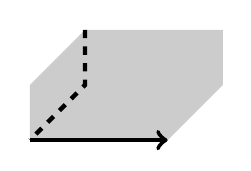
\begin{tikzpicture}[baseline, scale=0.7]
		\fill[gray!40] (0, 1) -- (-1, 0) -- (-1, -1) -- (1.5, -1) --(2.5, 0) -- (2.5, 1)  --cycle;
		\draw[ultra thick, dashed] (0,1) -- (0,0) -- (-1, -1);
		\draw[ultra thick, ->] (-1, -1) -- (1.5, -1);
	\end{tikzpicture} \;\Rightarrow \cdots \Rightarrow\; 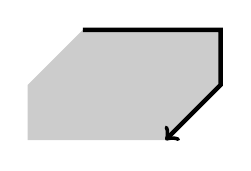
\begin{tikzpicture}[baseline, scale=0.7]
		\fill[gray!40] (-1, 1) -- (1.5, 1) -- (1.5, 0) -- (0.5, -1) -- (-2, -1) -- (-2, 0) --cycle;
		\draw[ultra thick, ->] (-1,1) -- (1.5 , 1) -- (1.5, 0)  -- (0.5, -1);
	\end{tikzpicture} \; =: \beth. \]

	Recall that
	$\cate{D}(\cdots)\times\cate{D}(\cdots)\to\cate{D}(\cdots)$ is absolute
	as a right Kan extension
	(Proposition~\ref{prop:localization-functor-abs}). Therefore the composite
% segment-id: o014.li2.chapter4.k-flat-derived-tensor-a.e003
	\begin{equation*}\begin{gathered}
		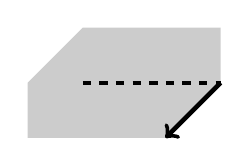
\begin{tikzpicture}[baseline=(O), scale=0.7]
			\fill[gray!40] (-1, 1) -- (1.5, 1) -- (1.5, 0) -- (0.5, -1) -- (-2, -1) -- (-2, 0) --cycle;
			\draw[ultra thick, dashed] (-1,0) -- (1.5, 0);
			\draw[ultra thick, ->] (1.5, 0)  -- (0.5, -1);
			\coordinate (O) at (0, 0);
		\end{tikzpicture}
		\quad \text{is the right Kan extension of $\beth$ along} \quad
		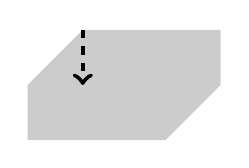
\begin{tikzpicture}[baseline=(O), scale=0.7]
			\fill[gray!40] (-1, 1) -- (1.5, 1) -- (1.5, 0) -- (0.5, -1) -- (-2, -1) -- (-2, 0) --cycle;
			\draw[ultra thick, dashed, ->] (-1, 1) -- (-1, 0);
			\coordinate (O) at (0, 0);
		\end{tikzpicture}.
	\end{gathered}\end{equation*}
	Applying the morphism into $\beth$ and the universal property of the right
	Kan extension (Definition~\ref{def:Kan-extension}) gives the desired
	$\alpha$.

	Once the existence of $\alpha$ has been established, take K-flat complexes
	as in the first paragraph of the proof and compute all the functors in the
	upper layer. This proves that $\alpha$ is an isomorphism.
\end{proof}

% segment-id: o014.li2.chapter4.k-flat-derived-tensor-a.p015
From now on, arguments of this kind based on universal properties will often
be omitted; instead, we shall verify statements directly using resolutions.
